% Created 2018-11-21 on. 17:00
\documentclass[11pt]{article}
\usepackage[utf8]{inputenc}
\usepackage[T1]{fontenc}
\usepackage{fixltx2e}
\usepackage{graphicx}
\usepackage{longtable}
\usepackage{float}
\usepackage{wrapfig}
\usepackage{rotating}
\usepackage[normalem]{ulem}
\usepackage{amsmath}
\usepackage{textcomp}
\usepackage{marvosym}
\usepackage{wasysym}
\usepackage{amssymb}
\usepackage{hyperref}
\usepackage{cite}
\usepackage{tikz}
\usepackage{tkz-euclide}
\usetikzlibrary{calc,patterns,angles,quotes}
\usetikzlibrary{decorations.pathreplacing}
%\usepackage[numbers]{natbib}
\usepackage[round]{natbib}



\usepackage{natbib}
\bibliographystyle{abbrvnat}
\setcitestyle{authoryear,open={[},close={]}}
\tolerance=1000
%\bibliography{semsteroppgave}
\usepackage[margin=1.0in]{geometry} \setlength\parindent{0pt}
\author{Christian O'Cadiz Gustad}
\date{\today}
\title{Semesteroppgave}
\hypersetup{
  pdfkeywords={},
  pdfsubject={},
  pdfcreator={Emacs 25.2.2 (Org mode 8.2.10)}}

\begin{document}

\maketitle


\label{sec-1}


\newpage
%\section*{Timeplaner}
%\label{sec-2}
%\begin{center}
%\begin{tabular}{l|l|l|r}
%Dato & Klasse & Varighet & Tidspunkt\\
%1.Nov & R2 & To timer & 13:00-14:30\\
%\hline
%Fag: & Kompetansemål:\\
%Matematikk & \\
% & \\
% & \\
%\hline
% &  &  & \\
% &  &  & \\
% &  &  & \\
% &  &  & \\
%\end{tabular}
%\end{center}
\subsection*{Første time}
\label{sec-2-1}
\begin{center}
\begin{tabular}{l|l|l|l}
Tid & Hva skjer? & Hvordan skal & Hvorfor skal\\
 &  & dette skje? & det skje?\\
\hline
0-3 & Oppstart av timen. & Få ro i klassen. & For å få oppmerksomheten\\
min &  & Elevene setter seg & og roen til elevene.\\
 &  & faste sitteplasser. & \\
 &  & Ta fravær ved at & \\
 &  & elevene krysser seg & \\
 &  & av. & \\
\hline
3-15 & Gjennomgang av temaet. & Elevene lytter og de & Dette skal skjer for\\
min & Læreren repiterer & som vil tar notater. & å formidle temaet.\\
 & tidligere matriale, & Først vil noen & Læreren vil stille\\
 & samt presentere & minutter bli satt & spørsmål på kritiske\\
 & elevene for & av tid til å snakke & punkter for å gi dem\\
 & skalarproduktet. & om vektorer og hva & en bedre forståelse\\
 &  & det vil si at vi har & samnt skape dialog\\
 &  & ett produkt av & i klassen. Deretter\\
 &  & vektorer. Deretter & forklares det hvordan\\
 &  & vil skalarproduktet & skalarproduktet vi\\
 &  & bli innført og & innfører nå, likner på\\
 &  & egenskapene til dette & skalarproduktet i\\
 &  & produktet bli forklart. & planet.\\
 &  & Så vil en & \\
 &  & eksempeloppgave & \\
 &  & bli gjennomgått. & \\
\hline
15-35 & Elevene arbeider med & Eleven jobber med & Dette gjøres for å\\
min & oppgaver de har ifra & oppgavene. Hvis noen & styrke elevens forståelse\\
 & ett ark Læreren har & ikke forstår oppgaven & av temaet som har blitt\\
 & lagd. Læreren går & eller trenger hjelp, & gjennomgang av læreren.\\
 & rundt og hjelper & rekker de opp hånda. & Dette gir også læreren\\
 & elevene med oppgavene. &  & mulighet til å gjengi noe\\
 &  &  & eleven ikke har forstått,\\
 &  &  & eller som  var uklart.\\
\hline
35-45 & Læreren vil gjennomgå & Læreren gjennomgår & Dette gjøres for\\
min & løsning på noen av de & oppgaver som elevene & konsolidering og gir i\\
 & oppgavene elevene & har slitt med eller de & tillegg en mulighet for\\
 & slet med. Samt gå & oppgavene som var mest & å oppklare noe elevene\\
 & igjennom hva timen & instruktive. Elevene & ikke har forstått.\\
 & handlet om. & vil fortsette å arbeide & \\
 &  & med tidligere oppgaver, & \\
 &  & dersom de ikke ønsker å & \\
 &  & følge gjennomgangen. & \\
\end{tabular}
\end{center}
\newpage
\subsection*{Andre time}
\label{sec-2-2}
\begin{center}
\begin{tabular}{l|l|l|l}
Tid & Hva skjer? & Hvordan skal & Hvorfor skal\\
 &  & dette skje? & det skje?\\
\hline
0-2 & Oppstart av timen. & Få ro i klassen etter & For å få oppmerksomheten\\
min &  & friminutt. Læreren vil & og roen til elevene.\\
 &  & få overblikk over hvem & \\
 &  & som er tilstedet. & \\
\hline
2-15 & Inroduksjon av & Etter elevene har & Dette gjøre for å\\
min & kryssprodukt. & fått roen, kan & formidle stoffet til\\
 &  & læreren gå igjennom & elevene. Spesielt viktig\\
 &  & prinsippene til & blir da den så kalte\\
 &  & kryssproduktet. & høyrehåndsregelen.\\
 &  & Slik som hvordan & Denne blir sentral i\\
 &  & kryss produktet & den geometriske\\
 &  & gir en vektor ffra & tolkningen av\\
 &  & to vektorer, & kryssproduktet.\\
 &  & i motsetning til & \\
 &  & skalarproduktet som & \\
 &  & gir ett tall. & \\
 &  & Deretter vil det bli & \\
 &  & gjennomgått hvilke & \\
 &  & egenskaper dette & \\
 &  & produktet har, og den & \\
 &  & geometriske tolkningen. & \\
\hline
15-35 & Arbeid med oppgaver. & Eleven jobber med & Oppgavene vil fokusere\\
min &  & oppgavene. Hvis noen & på regneregler og\\
 &  & ikke forstår oppgaven & determinant metode. I\\
 &  & eller trenger hjelp, & tilegg til formler for\\
 &  & rekker de opp hånda. & areal av trekanter.\\
\hline
35-45 & Oppgaver løst på & Læreren gjennomgår & Dette gjøres for\\
min & tavlen. & oppgaver som elevene & konsolidering og gir i\\
 &  & har slitt med eller & tillegg en mulighet for\\
 &  & oppgavene som var me & å oppklare noe elevene\\
 &  & instruktive. Elevene & ikke har forstått.\\
 &  & vil fortsette å arbe & \\
 &  & med tidligere oppgav & \\
 &  & dersom de ikke ønske & \\
 &  & følge gjennomgangen. & \\
 &  &  & \\
\end{tabular}
\end{center}
\newpage
\section*{Problemstillling semesteroppgaven}
Praksisskolen er en videregående skole i Oslo, som er fokusert på studiespesialserende men har også tilbud innen idrett og entreprenørskap. 
Min problemstilling går ut ifra en dobbelttime gjennomført på Kongshavn vidregående skole under praksis.
Timen er ment for en klasse på 14 elever i R2. Jeg har har valgt å fokusere på: <<Hvordan kan redskaper som 
digitale verktøy og illustrende oppgaver kan påvirke undervisningen og hjelpe elevene få en aha-opplevelse.>>   

\section{Beskrivelse av klassen og presentasjonen av undervisningsopplegget.}
\label{sec-1}

Klassen består av 14 elever som har valgt seg inn til faget R2 matematikk. Siden R2 er ett programfag vil en høyere andel av elevene være motiverte til å lære faget. Dette har jeg også fått intrykk av under tidligere observasjonstimer hos klassen. Strykprosenten sank i 2017 innen programfag matematikk samnt gjennomsnittskarakteren økte  med 0.2 karakterpoeng \href{https://www.udir.no/tall-og-forskning/finn-forskning/tema/karakterer/eksamenskarakterer-varen-2017/}{[Udir, 2017]}.\\

Kjønnsfordelingen i klassen er jevnt, og man får inntrykk av at jentene ligger jevnt over på ett høyere faglig nivå enn guttene. Noe som virker typisk ettersom jenter gjør det bedre i teoretisk matematikk i følge \href{https://www.udir.no/tall-og-forskning/finn-forskning/tema/karakterer/eksamenskarakterer-varen-2017/}{[Udir, 2017]}. Her er det spesielt er det en gjeng på 2-3 gutter som ikke gjør arbeidet de skal i de tidligere timene vi har observert. \\

Tidligere hadde klassen hatt prøve innen integrasjon og derivasjon av trigonometriske funksjoner. Etter å ha observert denne prøven kom det frem at noen av elevene slet mer enn de gav intrykk av. Spesielt ettersom flere vi så for oss var gode elever leverte en blank oppgave. Disse elevene slet med motivasjonen for faget, mens andre elever vi så for oss være svake viste seg å prestere sterkt på prøven.
Ellers virker klassemiljøet godt der det er liten annen problematferd. Det virker som om elevene har god relasjon til læreren og til hverandre.\\

I denne semestroppgaven vil jeg først beskrive oplegget samnt analysere og drøfte opplegget og resultatet ut fra pedagogisk og fagdidaktikks teori.

Den faste underviseren deres er en svært god lærer som har gitt ut flere bøker innen matematikk for videregående. Terskelen virker lav for at elevene skulle  komme med inspill og spørsmål til undervisningen. 
Strukturen på undervisningen hennes virker å gå som følger:
\begin{itemize}
\item \emph{7-15 min} Gå gjennom teori og eksempler på tavla.
\item \emph{20-28 min} Elevene får arbeide med oppgaver alene.
\item \emph{10 min} Læreren går igjennom vansklige og illustrerende oppgaver på tavla.
\end{itemize}
Vi bestemte oss derfor å holde oss til denne tidsplanen, men denne gangen med i en dobbeltime med to slike opplegg etter hverandre. Målet for den første undervisningstimen var å gjøre elevene kjent med skalarproduktet i dimensjon tre derved gjøre assimilasjon \citep{Saljo} av kjente bregreper. Deretter introdusere vektorproduktet i dimensjon tre, som vil være helt nytt i motsetning til skalarproduketet som elevene kjenner fra tidligere i dimensjon to. Dette skyldes at vektorproduktet ikke eksisterer i dimensjon 2.\\

Før denne timen har vi observert flere timer som læreren har holdt, samt holdt en dobbeltime der vi gikk igjennom vektorer og konstruksjoner i dimensjon tre.\\
Etter  timene under veiledning av denne læreren var det noen punkter hun anbefalte gjorde
\begin{itemize}
\item Lag egene oppgaver til elevene.
\item Planlegg hva som skal stå på tavla.
\end{itemize}
Vi bestemte oss derfor for å gjøre dette før timen, og hvordan dette ble utøvd vil forklart videre. Tidligere hadde en time vært holdt der læreren ikke hadde forbredt seg nok på hva som skulle stå på tavla og da observerte praksisveileder at flere av elevene slet med å ta notater.

\section{Presentasjon av undervisning opplegget}
\label{sec-2}
Undervsningsopplegget som skal drøftes er for en dobbeltime i R2 ett fag elevene selg har valgten derfor vil disse elvene være spesielt motiverte og vil være i stor grad derevet av indre motivasjon \citep{KletteH}. Dette gir læreren frihet og rom i undervisningen og kan gå igjennom ulike perspektiver på temaet \citep{Ball}.\\

Vårt format vil derfor være tradisjonell undervisning og vil bære preg av en behavioristisk tilnærming \citep{Saljo} til læring. Nemlig at læreren formidler ferdig kunnskap til elevene. Vi starter timen med å vise de geometriske 3D figurene vi lagde sist i Geogebra der vi snakket om trekanter, plan og vinkler i rommet. Dette brukes til å illustrere aspekter ved vektorer i 3 dimensjoner, der elevene er vandt med å jobbe i dimensjon to hvor det er langt enklere å tegne i boka. Dette vil også fungere som en gjennomgang av det de lærte forrige time og er et godt eksempel på en konsolideringsituasjon. Her illustrer vi vinkel begrepet samnt geometriske flater i rommet, dette vil være et typisk eksempel på utvikling av det kognitive skjemaet innen det konstruktivistiske  \citep{Saljo}. Etter elevene har gjort dette hoppet fra dimensjon to til dimensjon tre vil Vygotskijs \emph{proksimale utviklingssone} være etablert. Læreren påpeker hvordan begreper de kjenner til utvides til dimensjon tre. Skalar produktet blir da det naturlige startpunktet ettersom alt som kjennertegner det i dimensjon to også holder i dimensjon tre. 

Ved bruk av CAS Geogebra illustreres dette visuelt. Elevene virket som de likte hvordan dette verktøyet ble untyttet som står i samsvar med hva som sies i\citep{Heid}.\\

\begin{wrapfigure}{r}{0.45\textwidth}
 \begin{align}
\label{vec1}\vec{q} \cdot \vec{p} &= q_1p_1 + q_2p_2 + q_3p_3,\\
\label{vec2} \vec{q} \cdot \vec{p} &= 0 \Longleftrightarrow \vec{q} \perp \vec{p},\\
\label{vec3}\vec{q} \cdot \vec{p} &= |\vec{q}||\vec{p}|\cos{\theta}.
 \end{align}
 \begin{center}
   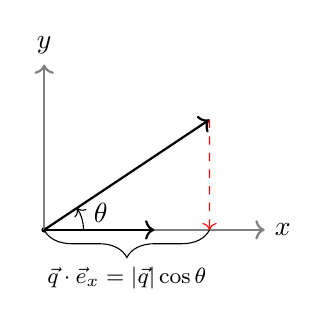
\begin{tikzpicture}[scale=0.7]
   \coordinate (origo) at (0,0);
   \coordinate (pivot) at (1,5);
   % draw axes
   \fill[black] (origo) circle (0.05);
   \draw[thick,gray,->] (origo) -- ++(4,0) node[black,right] {$x$};
   \draw[thick,gray,->] (origo) -- ++(0,3) node (mary) [black,above] {$y$};
   \draw[thick,->](origo) -- ++(2,0) coordinate (hund);
   \draw[thick,->] (origo) -- ++ (3,2) coordinate (bob);
   \pic [draw, ->, "$\theta$", angle eccentricity=1.5] {angle = hund--origo--bob};
   \draw [dashed,->,red] (bob) -- (3,0);
   \draw [decorate,decoration={brace,amplitude=10pt,mirror},xshift=0pt,yshift=0pt]
   (origo) -- (3,0) node [black,midway,below,yshift=-10pt]{\footnotesize $\vec{q}\cdot \vec{e}_x = |\vec{q}|\cos{\theta}$};
\end{tikzpicture}
 \end{center}
\end{wrapfigure}



Deretter setter vi i gang med introduksjon av skalarproduktet og de algebrasike egenskapene dette har. Dette vil mer eller mindre virke som repitisjon for dem fordi skalarproduktet i dimensjon 2 har de arbeidet med tidligere. Vi velger derfor å gå litt dypere inn i hva ett skalarprodukt er og hvordan man tolke det geometrisk.  
For det første holder vi oss til dimensjon 2 for å enklest forklare dette. Vi begynner med å tolke \eqref{vec3} i tilfellet der $\vec{p} = \vec{e}_x$, der $\vec{e}_x$ er enhetsvektoren i $x$ retning.  Formelen \eqref{vec3} følger da fra trigonometri elevene kjenner godt.
Vi får da følgende bildet som vist på siden. I dette tilfellet vil skalarproduktet gi lengded av projeksjonen til $\vec{p}$ ned på $x$-aksen. Dermed har elevene blitt forklart at indreproduktet mellom en vektor og en vektor med lengde en, definerer lengden av projeksjonen. Den generaliserte tolkningen blir de at skalarproduktet er den \emph{skalerte projeksjonen} av vektorene.
Dette er \emph{specialized content knowlage} i henhold til \citep{Ball} og er av typen \emph{conseptual understaning} i \emph{intertwined strands of proficientcy} modellen man finner i \citep{addup}. Denne typen kunnskap vil elevene ikke få utprøvd men illustrer hva som kommer i horisonten samnt gir nye perspektiver på skalarproduktet. Etter dette går læreren igjennom resten av teorien knyttet videre til skalarproduktet. Så jobber elevene med oppgaver ifra boka, mens læreren går rundt å hjelper de som trenger det. Elevene virker å ta oppgavene veldig rask og det er få som sliter med oppgavene.\\
\begin{wrapfigure}{r}{0.45\textwidth}
  \begin{center}
  \begin{align}
|\vec{a}\times \vec{b}|  & = |\vec{a}||\vec{b}| \sin{\theta},\\
\vec{a}\cdot (\vec{b}\times \vec{c}) & = \vec{b} \cdot(\vec{c} \times \vec{a})  = \vec{c}\cdot(\vec{a}\times \vec{b})
  \end{align}
  \includegraphics[scale = 0.4]{./img/cross.png}
    \end{center}
\end{wrapfigure}


Etter pausen kommer elevene tilbake ifra friminutt er det neste temaet som introduseres nemlig kryssproduktet. Læreren beskriver produktet og vektlegger at dette er noe som ikke fungerer i dimensjon 2 men noe som kan brukes is dimension 3\footnote{I dimensjon 7 finns også kryssproduktet, men jeg unnlot å nevne dette. Kanskje litt mye special content knowlage og mer forvirring.}. Høyrehåndsregelen blir gjennomgått, samnt de algebraiske egenskapene kryssproduktet. Deretter gjennomgår går vi igjennom formelen for kryssproduktet. Dette er som kjent en ganske stygg formel, og vi viser  de mer elegante likningene ved hjelp av detrminant metoden. Dette minner om \emph{Cover-Up method} man finner i \citep[side 273]{addup2}, men  her dekker man lager en 3x3 matrise der den øverste radene er basisvektorene  og vektorene skal krysses de 2 radene under. Deretter beregner man determinanten av denne matrisen, ved hjelp av linæralgebra over deres nivå. Her er det lett å gå i fella med fortegn, dette merket man også på elevene som tidvis gjorde denne feilen. Det var ikke fasit på alle oppgavene og dette ble ett problem at elevene gjorde denne feilen uten å merke seg det selv.




Vi deler ut egen lagde oppgaver der vi har lagd noen egene som spesielt illustrer regelen om at lendgen av kyrrsproduktet mellom to vektorer tilsvarer arealet av paralellorgrammet vektorene spenner. Vi velger derfor å gi dem følgende oppgave:
\subsection*{Oppgave}

Bruk kryssproduktet til å finne arealet av trekanten:  

\begin{center}
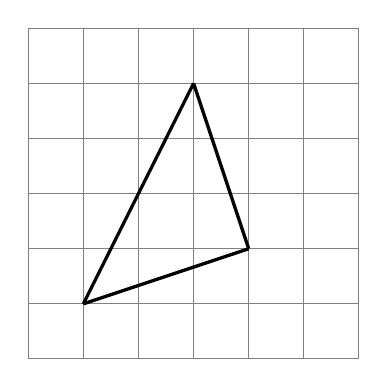
\begin{tikzpicture}[scale = 0.7,every node/.style={scale=0.7}]
\tkzInit[xmin=-1,xmax=5,ymin=-1,ymax=5]
\tkzGrid[color=gray]
\tkzAxeXY[very thick]
\draw[black,very thick] (3,1) -- (2,4);
\draw[black,very thick] (3,1) -- (0,0);
\draw[black,very thick] (2,4) -- (0,0);
--cycle;
\end{tikzpicture}    
\end{center}


Dette er en rik oppgave \citep{rike} siden den også kan løses ved hjelp av sinus setningen. Dette sitter kanskje litt dypt inne hos elevene og vil virke vanskelig, mens ved hjelp av reglene til kryssproduktet virker dette enklere. Først må eleven gjenkjenne at disse 2 dimensjonale vektorene kan tolkes som vektorer i rommet. Deretter beregne kryssproduktet av disse vektoren. Så regne ut lengden av kryssproduktet som gir det dobbelte av arealet til trekanten. Dette vil gi at  arealet av trekanten er 5.  
%\section{Analyse av undervisningsopplegget i teori og utførelse}
%\label{sec-3}



\section{Refleksjon}


\label{sec-4}
% Emacs 25.2.2 (Org mode 8.2.10)
\newpage
\bibliography{semesteroppgave}
\end{document}